\chapter{Metodologia}
\label{cap:metodologia}
Este capítulo apresenta a metodologia e os recursos utilizados para atingir o objetivo do trabalho.

\section{Visão geral}
\begin{figure}[h]
    \centering
    \caption{Etapas de desenvolvimento da pesquisa}
    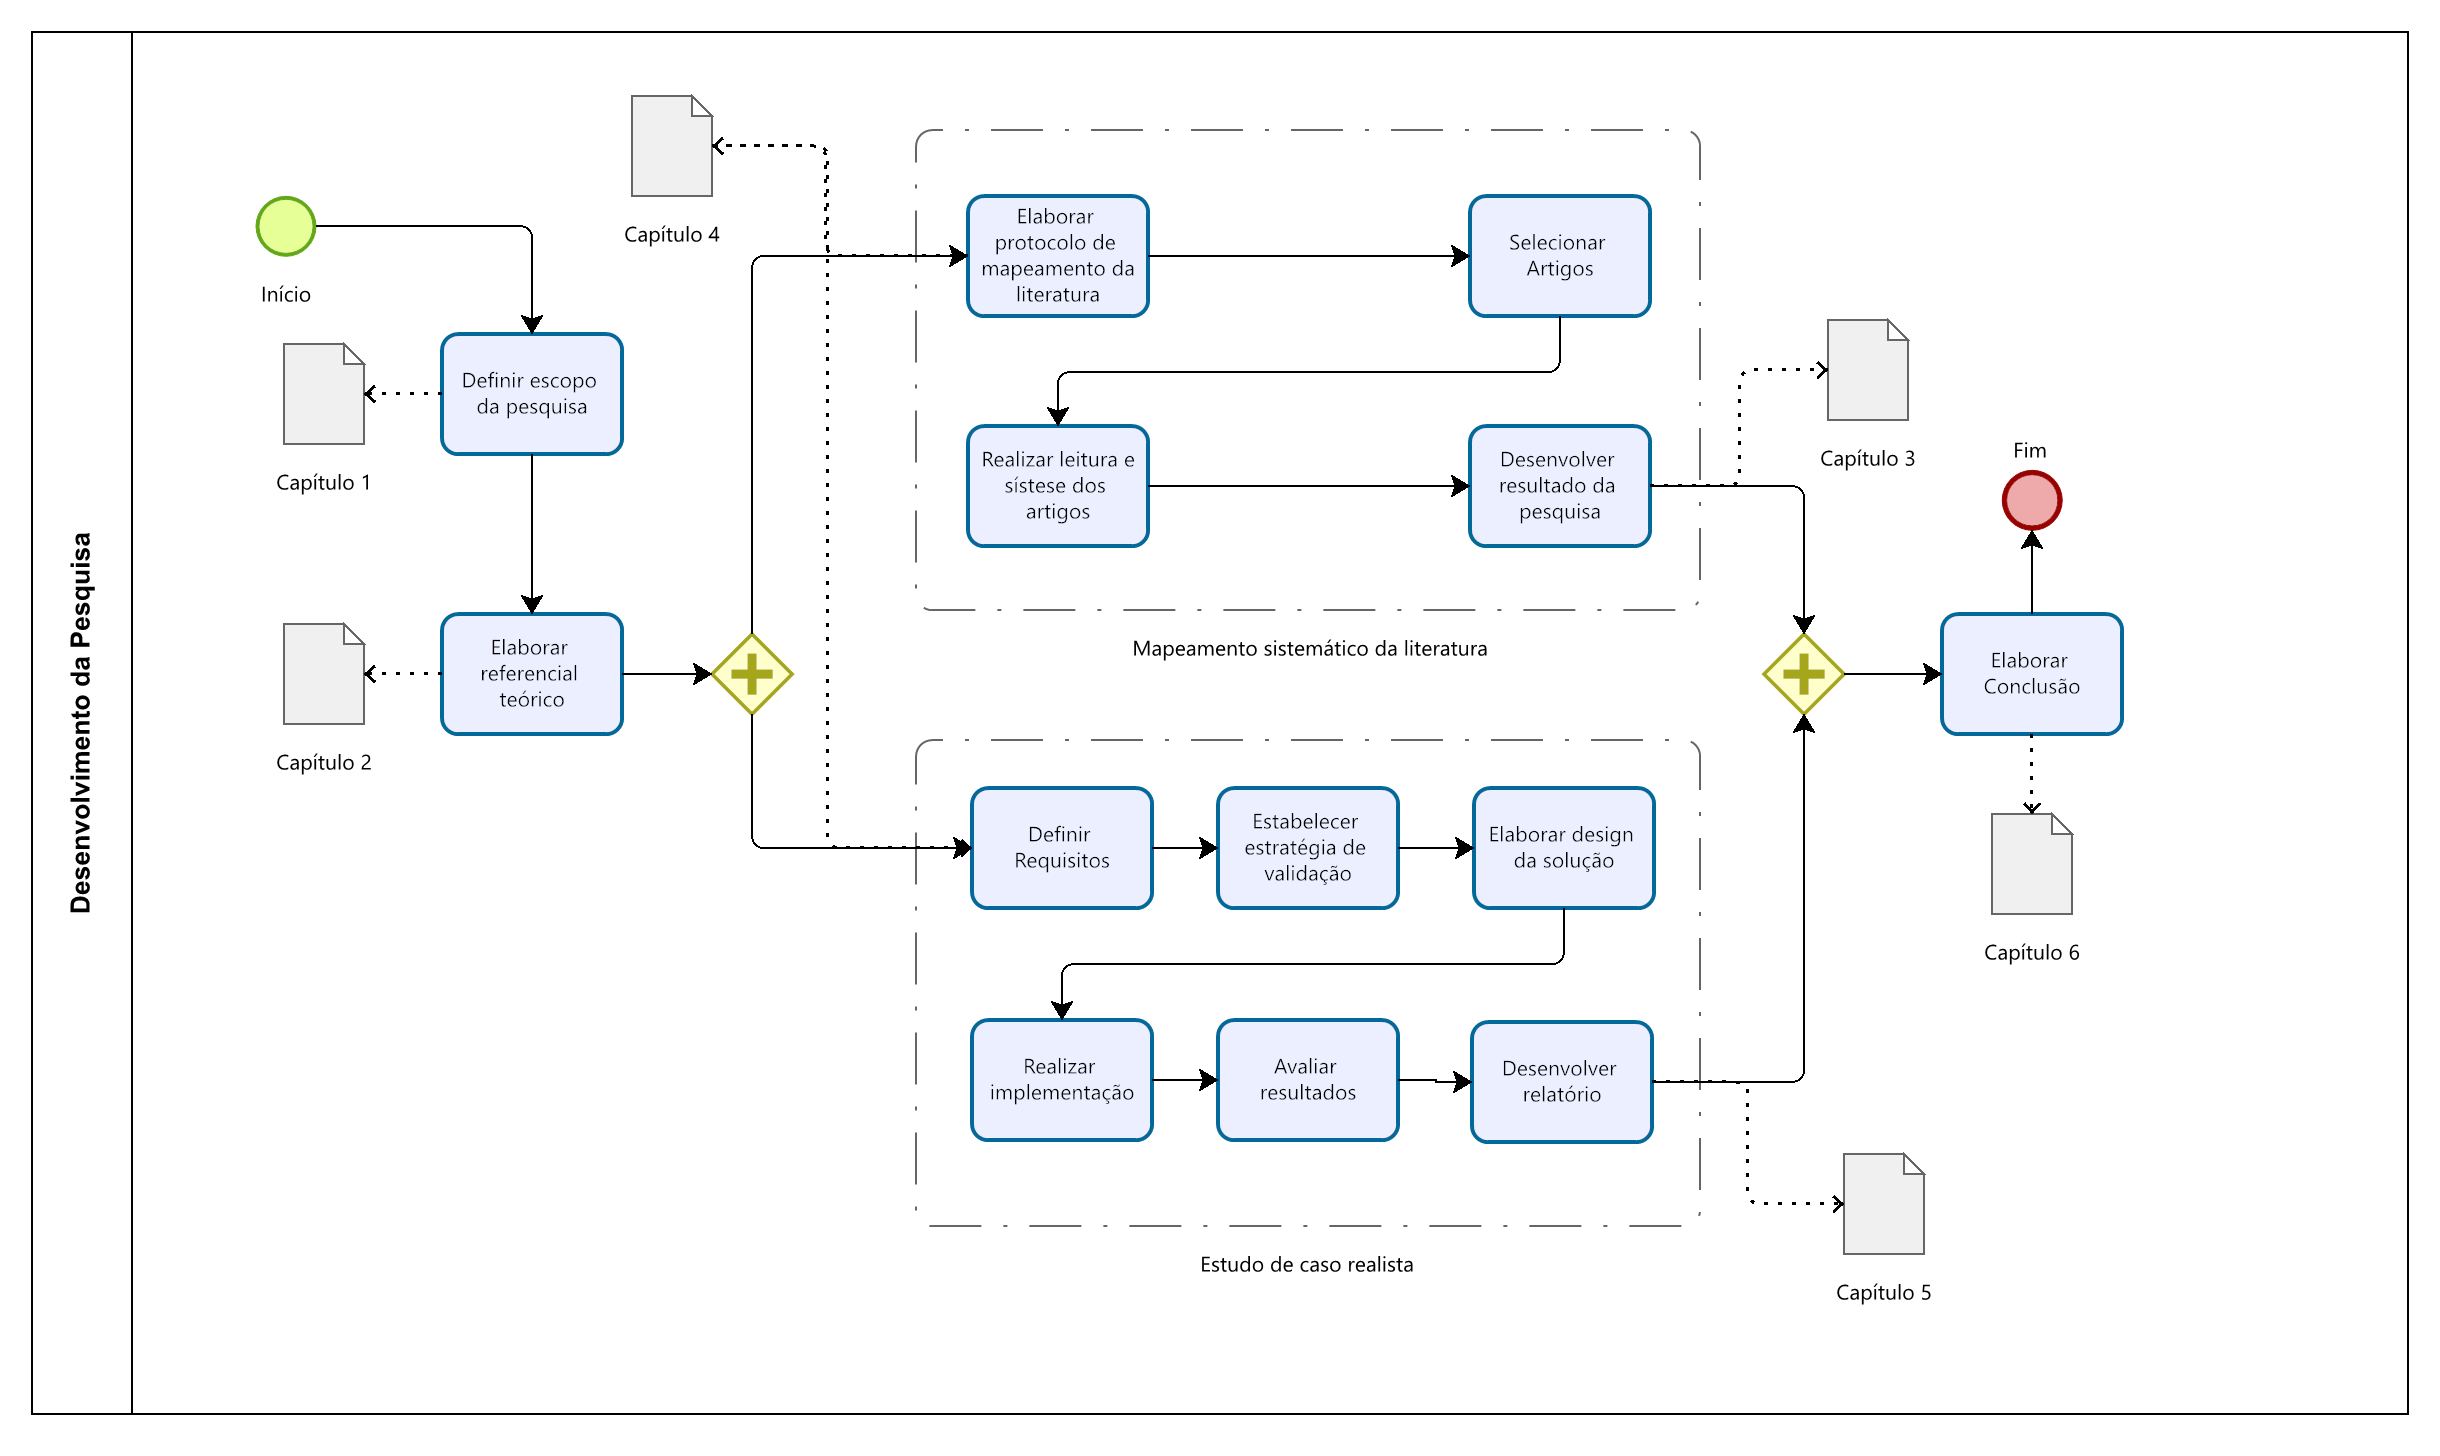
\includegraphics[width=0.9\textwidth]{media/bpmn_metodo_recurso.png}
    \legend{Fonte: o autor}
    \label{fig:metodo_recurso}
\end{figure}

Pode-se observar na \autoref{fig:metodo_recurso} as etapas de execução dessa pesquisa. Inicialmente, o escopo é definido e primeiro capítulo é elaborado. Em seguida, a fundamentação teórica com os conceitos-chave é construída. Posteriormente, se realiza um mapeamento da literatura buscando trabalhos similares. Adicionalmente, um estudo de caso realista com a utilização de microsserviços e diversos conceitos do \acrshort{ddd} é desenvolvido e um relatório é produzido. Por fim, é escrita a conclusão do trabalho.

\section{Mapeamento sistemático da Literatura}
Esta seção apresenta o protocolo de mapeamento sistemático da literatura usado para atingir os objetivos da pesquisa.

\subsection{Questões de pesquisa}
\label{section:questoes_pesquisa}
\begin{enumerate}
    \item[Q1:] Quais são as principais estratégias para elaboração de sistemas com microsserviços e \acrshort{ddd}?
    \item[Q2:] Quais são os principais desafios na utilização de \acrshort{ddd} como estratégia de delimitação de microsserviços?
    \item[Q2:] Quais são os anti-padrões a serem evitados na utilização de \acrshort{ddd} com microsserviços?
    
\end{enumerate}

\subsection{Estratégia de busca}
Esta seção apresenta a estratégia de buscas de artigos científicos e livros relacionados à pesquisa. As ferramentas utilizadas para realizar as buscas são:
\begin{itemize}
    \item \textbf{Periódicos Capes:} É uma ferramenta disponibilizada pelo governo federal para uso de estudantes e pesquisadores. Acessando através da instituição de ensino ou pesquisa, é possível ter acesso completo a uma grande quantidade de artigos científicos publicados em variadas revistas, conferências e universidades. A principal vantagem dessa ferramenta é a possibilidade de ler o conteúdo integral de grande parte das publicações disponíveis. Por outro lado, as expressões de busca atualmente suportadas são bem limitadas.
    \item \textbf{\english{Scopus:}} Trata-se de um ferramenta similar ao Periódicos Capes. No entanto, o \english{Scopus} permite a elaboração de expressões de buscas mais complexas e sofisticadas, servindo para descobrir publicações não detectadas pelas outras plataformas. Além disso, possui um acervo bem mais amplo que o Periódicos Capes. Entretanto, algumas publicações não podem ser vistas na íntegra de forma gratuita.
    \item \textbf{\english{Google Docs:}} Ferramenta desenvolvida pela \english{Google LLC} que permite a criação e edição de documentos de texto. Suas grandes vantagens em relação a ferramentas de outros fornecedores são as avançadas ferramentas de colaboração e a possibilidade de acesso por meio de navegadores \english{web}, sem necessidade de instalação de \english{software} específico.
    \item \textbf{\english{Google Sheets}}: Com as mesmas características e vantagens do \english{Google Docs}, essa ferramenta fornece recursos para elaboração de planilhas de cálculo. É muito útil para realizar análise de dados simples e também visualizar e apresentar dados tabulares.
\end{itemize}

Como grande parte das publicações na área de computação são em inglês, esta pesquisa utiliza esse idioma para fazer buscas nas ferramentas indicadas. Além disso, \acrfull{ams} e \acrfull{ddd} são relativamente recentes, as buscas se limitaram a publicações feitas nos últimos 20 anos.

Os termos-chave para realização das buscas são: Microsserviço, \acrshort{ddd} e \acrlong{ddd}. Como a busca será feita em inglês, se usará \english{microservice} nas buscas.
\subsection{Expressão de busca}
\label{section:string_busca}

\begin{quadro}[H]
\centering

\setlength{\tabcolsep}{0.8em} % for the horizontal padding
\renewcommand{\arraystretch}{1.5}% for the vertical padding
\caption{Expressão de busca utilizada}
\begin{tabular}{|p{4.5in}|}

\hline
Expressão de Busca \\ \hline
\english{( ( TITLE-ABS-KEY ( microservice ) AND TITLE-ABS-KEY ( domain-driven AND design ) ) OR ( TITLE-ABS-KEY ( microservice ) AND TITLE-ABS-KEY ( ddd ) ) )} \\ \hline

\end{tabular}
\label{quad:string_busca}
\fonte{o autor}
\end{quadro}

No \autoref{quad:string_busca}, percebe-se que a expressão de busca pretende retornar todas as publicações que contenham as palavras chaves no título, resumo ou na seção de \english{keywords}.

\subsection{Estratégia de seleção}
A seguir são apresentados critérios para inclusão de publicações na pesquisa.
\label{section:criterios_inclusao}
\begin{itemize}
    \item Texto completo disponível de forma gratuita pelo portal Periódicos Capes.
    \item Materiais relacionados ao tópico de interesse, ou seja, título ou resumo.
    \item Publicações com ao menos 5 citações.
\end{itemize}

Por outro lado, estes são os critérios para exclusão de publicações.
\label{section:criterios_exclusao}
\begin{itemize}
    \item Publicações duplicadas.
    \item Materiais que não dispõem de informação relevante para responder às questões de pesquisa.
\end{itemize}

\subsection{Estratégia para extração de dados e análise}
Para atingir o objetivo do mapeamento da literatura, são filtrados manualmente nos artigos selecionados segundo os critérios de inclusão e exclusão. A partir da listagem reduzida, todas as publicações são lidas de forma integral.
Adicionalmente, todos os gráficos e tabelas nos artigos selecionados são avaliados visando extrair algum dado que permita realizar a comparação entre aspectos quantitativos das estratégias como, tempo de resposta, latência e taxa de transferência.

Informações qualitativas como recomendações, destaques, conceitos e estudos de casos são registrados em um documento no \english{\href{https://docs.google.com/document/d/1-dXE9_2-CtfDePG9Opkcyipq0F0dcYJ-Z_gbhi_qDhs/edit?usp=sharing}{Google Docs}}. Dados quantitativos como taxa de transferência, latência, tempo de processamento são armazenados em uma planilha no \english{\href{https://docs.google.com/spreadsheets/d/1R-PbCisie8QHARzF2rYtDx8UPOWksEeH-6-SEqIOTLg/edit?usp=sharing}{Google Sheets}}. 

A pesquisa é executada seguindo os passos a seguir:
\begin{enumerate}
    \item As expressões de busca citadas são inseridas nas ferramentas mencionadas.
    \item É feito o armazenamento das publicações retornadas em uma \href{https://docs.google.com/spreadsheets/d/1rtH8Jl1EHguqZ4Py2mgV3pab7IQzt72-Sv2S1jPzLsQ/edit?usp=sharing}{planilha de cálculo}.
    \item As publicações retornadas são filtradas conforme os critérios de inclusão e exclusão.
    \item Em cada artigo selecionado, é realizada a extração dos dados relevantes para responder às questões de pesquisa.
    \item Finalmente, são produzidas respostas para questões de pequisa com as informações extraídas das publicações.
\end{enumerate}

\section{Estudo de Caso}

\subsection{Contexto}
\label{section:contexto}
O estudo de caso é realizado em uma empresa fictícia chamada \emph{CarroFacil}. Essa empresa é uma locadora de veículos que atua em todo o território nacional. A empresa possui uma frota de veículos própria. A \emph{CarroFacil} possui uma grande quantidade de clientes, sendo pessoas físicas ou jurídicas. Eles podem alugar veículos por períodos de tempo variados, desde horas até semanas. Os veículos são retirados em uma das lojas da empresa. A \emph{Locadora de Veículos} possui um sistema de locação de veículos que foi desenvolvido há alguns anos e está apresentando problemas de escalabilidade e manutenção. Por esse motivo, a empresa decidiu desenvolver um novo sistema de locação de veículos utilizando microsserviços e \acrshort{ddd}.

\subsection{Processo de Desenvolvimento}
\label{section:processo_desenvolvimento}
O processo de desenvolvimento utilizado para construir o sistema de locação de veículos é o \english{Kanban}. Essa metodologia de desenvolvimento ágil é baseada em um quadro de tarefas, no qual cada tarefa é representada por um cartão \cite{gomes2014agile}. O quadro é dividido em colunas que representam o estado atual de cada tarefa. As colunas mais comuns são: \english{To Do}, \english{Doing} e \english{Done}. O quadro é atualizado conforme as tarefas são realizadas. A \autoref{fig:kanban} apresenta um exemplo de quadro \english{Kanban}.

\begin{figure}[h]
    \centering
    \caption{Exemplo de quadro \english{Kanban}}
    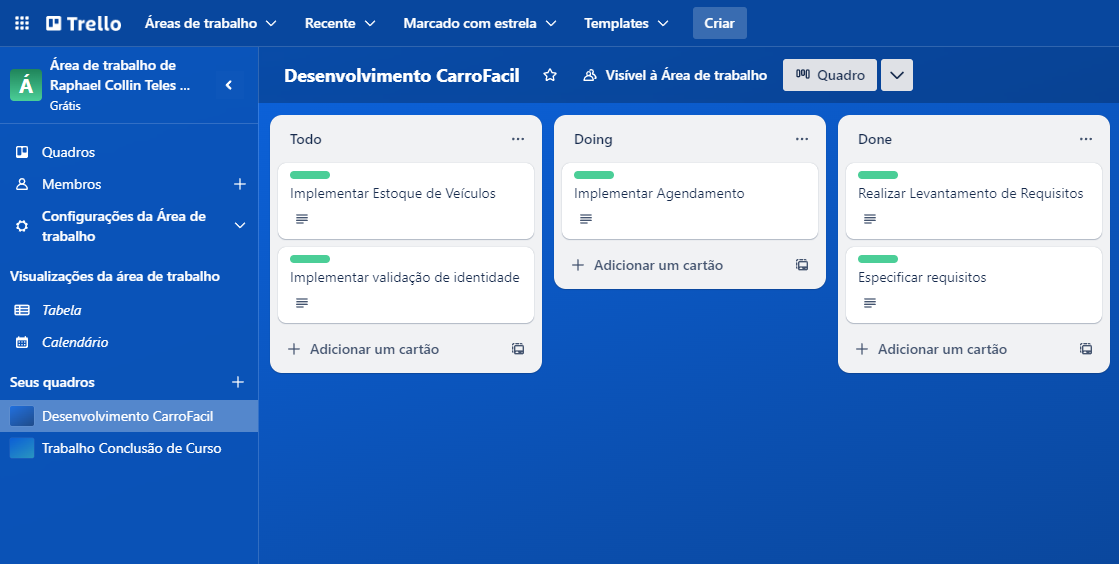
\includegraphics[width=0.9\textwidth]{media/kanban.png}
    \legend{Fonte: o autor}
    \label{fig:kanban}
\end{figure}

\subsection{Requisitos}
A seguir são apresentados os requisitos do sistema de locação de veículos.
\subsubsection{Requisitos Funcionais}

\subsubsection{Requisitos não Funcionais}

\subsection{Design}
Para realização do Design deste projeto, é utilizado o \english{Astah UML}. Com essa ferramenta, são criados diagramas de classes, diagramas de sequência, diagramas de casos de uso, entre outros diagramas da \english{\acrfull{uml}} \cite{astahUml}. Além disso, para modelagem da arquitetura do sistema, o modelo C4 é empregado. Este, pode ser entendido como um conjunto hierárquico de diagramas que possibilita a visão do sistema em diferentes níveis de abstração \cite{c4Model}. 

Para construção de cada microsserviços, é feito uso da \hyperref[section:hexagonal]{Arquitetura Hexagonal}  Essa, por sua vez, separa a aplicação em duas partes principais: núcleo da aplicação e adaptadores. O núcleo da aplicação contém as regras de negócio e os adaptadores são responsáveis por adaptar a aplicação para o mundo externo. Para modelagem do domínio, é utilizado o \english{\acrfull{ddd}}. O \acrshort{ddd} fornece uma estratégia para modelagem do domínio de negócio, diversos padrões para resolver problemas de modelagem recorrentes e facilidade de entendimento e manutenção de código \cite{evans2004ddd}.

\subsection{Implementação}
A implementação desse projeto é feita utilizando a linguagem de programação \english{Java} na versão 17. Para construção dos microsserviços, é utilizado o \english{framework} \english{Spring Boot}. Essa ferramenta fornece uma série de recursos para construção de microsserviços, como: injeção de dependências, configuração de banco de dados, configuração de \english{logs}, entre outros \cite{springBoot}. 

São utilizados dois banco de dados para armazenamento dos dados do sistema. O primeiro é um banco de dados relacional, que armazena dados de reservas. O segundo é um banco de dados não relacional, que armazena dados de clientes, veículos, entre outros. Para o banco de dados relacional, é utilizado o \english{PostgreSQL}. Para o banco de dados não relacional, foi escolhido o \english{Amazon DynamoDB}.

O \english{PostgreSQL} é um sistema de gerenciamento de banco de dados relacional de código aberto. Esse banco de dados é um dos mais populares do mundo, sendo utilizado por diversas empresas, como: \english{Apple}, \english{Cisco}, \english{Red Hat}, \english{Juniper Networks}, \english{Skype}, \english{Instagram}, \english{Spotify}, \english{Netflix}, entre outras \cite{postgreSql}. Trata-se de um banco de dados escalável, confiável, fácil de usar e com suporte a transações \acrshort{acid}.

Por outro lado, o \english{Amazon DynamoDB} é um banco de dados não relacional, que fornece desempenho de milissegundos de um dígito a qualquer escala. Esse banco de dados é totalmente gerenciado, ou seja, não é necessário realizar a configuração de servidores, escalabilidade, replicação, entre outros. Além disso, o \english{Amazon DynamoDB} é um banco de dados sem servidor, ou seja, o usuário paga apenas pelo que utiliza \cite{dynamoDb}.

Para a intercomunicação entre os microsserviços de maneira assíncrona, é utilizado o \english{Amazon SQS}. Esse \english{broker} de mensagens permite que os microsserviços se comuniquem de maneira assíncrona, sem que um microsserviço precise conhecer o outro \cite{amazonSqs}. Além disso, o \english{Amazon SQS} permite que as mensagens sejam armazenadas em uma fila, caso o microsserviço que as recebeu esteja fora do ar.

\subsection{Validação}
O projeto é desenvolvido com as estratégias de \acrfull{tdd} e \acrfull{bdd}. Essas abordagens de desenvolvimento de \english{software} permitem que o código seja desenvolvido de maneira mais confiável e com maior qualidade \cite{barauna2020tdd}. Além disso, o \acrshort{tdd} e o \acrshort{bdd} permitem que o código seja desenvolvido de maneira mais rápida, pois os testes são escritos antes do código.

Três tipos de testes são escritos para validar o sistema: testes unitários, testes de integração e testes de aceitação. Os testes unitários são escritos para validar métodos e classes do sistema. Por outro lado, os testes de integração validam a integração entre dois microsserviços e integrações com componentes externos, como banco de dados. Por fim, os testes de aceitação são implementados para validar os requisitos do sistema. É importante ressaltar que todos os testes são automatizados utilizando o \english{JUnit}.

\subsection{Implantação}
O sistema é implantado na nuvem da \english{\acrfull{aws}}. A \acrshort{aws} é uma plataforma de computação em nuvem que oferece mais de 200 serviços completos de datacenters em todo o mundo \cite{aws}. Esses serviços incluem computação, armazenamento, banco de dados, \english{networking}, \english{analytics}, \english{machine learning}, inteligência artificial, \english{Internet of Things}, segurança, entre outros.

Cada microsserviço é implantado em um \english{container} \english{Docker}. Essa tecnologia permite que os microsserviços sejam executados de maneira isolada, sem que um microsserviço interfira no outro. Além disso, o \english{Docker} permite que os microsserviços sejam executados em qualquer ambiente, sem que seja necessário realizar alterações no código \cite{docker}. O serviço \english{Amazon ECS} é utilizado para orquestrar os \english{containers} \english{Docker}. Esse serviço permite que os \english{containers} sejam executados em um ambiente de produção de maneira escalável e confiável \cite{amazonEcs}.

Um \english{cluster} \english{PostgreSQL} com o auxilío do serviço \english{Amazon RDS} é utilizado. Por outro lado, o \english{Amazon DynamoDB} e o \english{Amazon SQS} são soluções nativas da \acrshort{aws}.

Para a orchestração e automatização do provisonamento e configuração da infraestrutura, é feito uso da ferramenta \english{Terraform}. Essa ferramenta permite que a infraestrutura seja definida como código, ou seja, é possível definir a infraestrutura utilizando uma linguagem de programação \cite{terraform}. Além disso, o \english{Terraform} permite que a infraestrutura seja provisionada e configurada de maneira automatizada.